% Options for packages loaded elsewhere
\PassOptionsToPackage{unicode}{hyperref}
\PassOptionsToPackage{hyphens}{url}
%
\documentclass[
]{article}
\usepackage{amsmath,amssymb}
\usepackage{iftex}
\ifPDFTeX
  \usepackage[T1]{fontenc}
  \usepackage[utf8]{inputenc}
  \usepackage{textcomp} % provide euro and other symbols
\else % if luatex or xetex
  \usepackage{unicode-math} % this also loads fontspec
  \defaultfontfeatures{Scale=MatchLowercase}
  \defaultfontfeatures[\rmfamily]{Ligatures=TeX,Scale=1}
\fi
\usepackage{lmodern}
\ifPDFTeX\else
  % xetex/luatex font selection
\fi
% Use upquote if available, for straight quotes in verbatim environments
\IfFileExists{upquote.sty}{\usepackage{upquote}}{}
\IfFileExists{microtype.sty}{% use microtype if available
  \usepackage[]{microtype}
  \UseMicrotypeSet[protrusion]{basicmath} % disable protrusion for tt fonts
}{}
\makeatletter
\@ifundefined{KOMAClassName}{% if non-KOMA class
  \IfFileExists{parskip.sty}{%
    \usepackage{parskip}
  }{% else
    \setlength{\parindent}{0pt}
    \setlength{\parskip}{6pt plus 2pt minus 1pt}}
}{% if KOMA class
  \KOMAoptions{parskip=half}}
\makeatother
\usepackage{xcolor}
\usepackage[margin=1in]{geometry}
\usepackage{color}
\usepackage{fancyvrb}
\newcommand{\VerbBar}{|}
\newcommand{\VERB}{\Verb[commandchars=\\\{\}]}
\DefineVerbatimEnvironment{Highlighting}{Verbatim}{commandchars=\\\{\}}
% Add ',fontsize=\small' for more characters per line
\usepackage{framed}
\definecolor{shadecolor}{RGB}{248,248,248}
\newenvironment{Shaded}{\begin{snugshade}}{\end{snugshade}}
\newcommand{\AlertTok}[1]{\textcolor[rgb]{0.94,0.16,0.16}{#1}}
\newcommand{\AnnotationTok}[1]{\textcolor[rgb]{0.56,0.35,0.01}{\textbf{\textit{#1}}}}
\newcommand{\AttributeTok}[1]{\textcolor[rgb]{0.13,0.29,0.53}{#1}}
\newcommand{\BaseNTok}[1]{\textcolor[rgb]{0.00,0.00,0.81}{#1}}
\newcommand{\BuiltInTok}[1]{#1}
\newcommand{\CharTok}[1]{\textcolor[rgb]{0.31,0.60,0.02}{#1}}
\newcommand{\CommentTok}[1]{\textcolor[rgb]{0.56,0.35,0.01}{\textit{#1}}}
\newcommand{\CommentVarTok}[1]{\textcolor[rgb]{0.56,0.35,0.01}{\textbf{\textit{#1}}}}
\newcommand{\ConstantTok}[1]{\textcolor[rgb]{0.56,0.35,0.01}{#1}}
\newcommand{\ControlFlowTok}[1]{\textcolor[rgb]{0.13,0.29,0.53}{\textbf{#1}}}
\newcommand{\DataTypeTok}[1]{\textcolor[rgb]{0.13,0.29,0.53}{#1}}
\newcommand{\DecValTok}[1]{\textcolor[rgb]{0.00,0.00,0.81}{#1}}
\newcommand{\DocumentationTok}[1]{\textcolor[rgb]{0.56,0.35,0.01}{\textbf{\textit{#1}}}}
\newcommand{\ErrorTok}[1]{\textcolor[rgb]{0.64,0.00,0.00}{\textbf{#1}}}
\newcommand{\ExtensionTok}[1]{#1}
\newcommand{\FloatTok}[1]{\textcolor[rgb]{0.00,0.00,0.81}{#1}}
\newcommand{\FunctionTok}[1]{\textcolor[rgb]{0.13,0.29,0.53}{\textbf{#1}}}
\newcommand{\ImportTok}[1]{#1}
\newcommand{\InformationTok}[1]{\textcolor[rgb]{0.56,0.35,0.01}{\textbf{\textit{#1}}}}
\newcommand{\KeywordTok}[1]{\textcolor[rgb]{0.13,0.29,0.53}{\textbf{#1}}}
\newcommand{\NormalTok}[1]{#1}
\newcommand{\OperatorTok}[1]{\textcolor[rgb]{0.81,0.36,0.00}{\textbf{#1}}}
\newcommand{\OtherTok}[1]{\textcolor[rgb]{0.56,0.35,0.01}{#1}}
\newcommand{\PreprocessorTok}[1]{\textcolor[rgb]{0.56,0.35,0.01}{\textit{#1}}}
\newcommand{\RegionMarkerTok}[1]{#1}
\newcommand{\SpecialCharTok}[1]{\textcolor[rgb]{0.81,0.36,0.00}{\textbf{#1}}}
\newcommand{\SpecialStringTok}[1]{\textcolor[rgb]{0.31,0.60,0.02}{#1}}
\newcommand{\StringTok}[1]{\textcolor[rgb]{0.31,0.60,0.02}{#1}}
\newcommand{\VariableTok}[1]{\textcolor[rgb]{0.00,0.00,0.00}{#1}}
\newcommand{\VerbatimStringTok}[1]{\textcolor[rgb]{0.31,0.60,0.02}{#1}}
\newcommand{\WarningTok}[1]{\textcolor[rgb]{0.56,0.35,0.01}{\textbf{\textit{#1}}}}
\usepackage{graphicx}
\makeatletter
\newsavebox\pandoc@box
\newcommand*\pandocbounded[1]{% scales image to fit in text height/width
  \sbox\pandoc@box{#1}%
  \Gscale@div\@tempa{\textheight}{\dimexpr\ht\pandoc@box+\dp\pandoc@box\relax}%
  \Gscale@div\@tempb{\linewidth}{\wd\pandoc@box}%
  \ifdim\@tempb\p@<\@tempa\p@\let\@tempa\@tempb\fi% select the smaller of both
  \ifdim\@tempa\p@<\p@\scalebox{\@tempa}{\usebox\pandoc@box}%
  \else\usebox{\pandoc@box}%
  \fi%
}
% Set default figure placement to htbp
\def\fps@figure{htbp}
\makeatother
\setlength{\emergencystretch}{3em} % prevent overfull lines
\providecommand{\tightlist}{%
  \setlength{\itemsep}{0pt}\setlength{\parskip}{0pt}}
\setcounter{secnumdepth}{-\maxdimen} % remove section numbering
\usepackage{bookmark}
\IfFileExists{xurl.sty}{\usepackage{xurl}}{} % add URL line breaks if available
\urlstyle{same}
\hypersetup{
  pdftitle={Statistical analysis of the effect of environmental variables on abundance of flounder},
  pdfauthor={Olga Lyashevska},
  hidelinks,
  pdfcreator={LaTeX via pandoc}}

\title{Statistical analysis of the effect of environmental variables on
abundance of flounder}
\author{Olga Lyashevska}
\date{2024-10-31}

\begin{document}
\maketitle

{
\setcounter{tocdepth}{2}
\tableofcontents
}
\begin{Shaded}
\begin{Highlighting}[]
\CommentTok{\# load packages }
\NormalTok{packages }\OtherTok{\textless{}{-}} \FunctionTok{c}\NormalTok{(}\StringTok{"ggplot2"}\NormalTok{, }\StringTok{"MASS"}\NormalTok{, }\StringTok{"rmarkdown"}\NormalTok{, }\StringTok{"tinytex"}\NormalTok{, }\StringTok{"reshape2"}\NormalTok{, }\StringTok{"glmmTMB"}\NormalTok{, }\StringTok{"DHARMa"}\NormalTok{, }\StringTok{"emmeans"}\NormalTok{)}
\FunctionTok{lapply}\NormalTok{(packages, library, }\AttributeTok{character.only =} \ConstantTok{TRUE}\NormalTok{)}
\end{Highlighting}
\end{Shaded}

\begin{verbatim}
## This is DHARMa 0.4.7. For overview type '?DHARMa'. For recent changes, type news(package = 'DHARMa')
\end{verbatim}

\begin{verbatim}
## Welcome to emmeans.
## Caution: You lose important information if you filter this package's results.
## See '? untidy'
\end{verbatim}

\begin{verbatim}
## [[1]]
## [1] "ggplot2"   "stats"     "graphics"  "grDevices" "utils"     "datasets" 
## [7] "methods"   "base"     
## 
## [[2]]
## [1] "MASS"      "ggplot2"   "stats"     "graphics"  "grDevices" "utils"    
## [7] "datasets"  "methods"   "base"     
## 
## [[3]]
##  [1] "rmarkdown" "MASS"      "ggplot2"   "stats"     "graphics"  "grDevices"
##  [7] "utils"     "datasets"  "methods"   "base"     
## 
## [[4]]
##  [1] "tinytex"   "rmarkdown" "MASS"      "ggplot2"   "stats"     "graphics" 
##  [7] "grDevices" "utils"     "datasets"  "methods"   "base"     
## 
## [[5]]
##  [1] "reshape2"  "tinytex"   "rmarkdown" "MASS"      "ggplot2"   "stats"    
##  [7] "graphics"  "grDevices" "utils"     "datasets"  "methods"   "base"     
## 
## [[6]]
##  [1] "glmmTMB"   "reshape2"  "tinytex"   "rmarkdown" "MASS"      "ggplot2"  
##  [7] "stats"     "graphics"  "grDevices" "utils"     "datasets"  "methods"  
## [13] "base"     
## 
## [[7]]
##  [1] "DHARMa"    "glmmTMB"   "reshape2"  "tinytex"   "rmarkdown" "MASS"     
##  [7] "ggplot2"   "stats"     "graphics"  "grDevices" "utils"     "datasets" 
## [13] "methods"   "base"     
## 
## [[8]]
##  [1] "emmeans"   "DHARMa"    "glmmTMB"   "reshape2"  "tinytex"   "rmarkdown"
##  [7] "MASS"      "ggplot2"   "stats"     "graphics"  "grDevices" "utils"    
## [13] "datasets"  "methods"   "base"
\end{verbatim}

\begin{Shaded}
\begin{Highlighting}[]
\NormalTok{knitr}\SpecialCharTok{::}\NormalTok{opts\_chunk}\SpecialCharTok{$}\FunctionTok{set}\NormalTok{(}\AttributeTok{fig.path =} \StringTok{"figure/"}\NormalTok{, }\AttributeTok{dev =} \StringTok{"png"}\NormalTok{)}
\FunctionTok{set.seed}\NormalTok{(}\DecValTok{123}\NormalTok{)}
\end{Highlighting}
\end{Shaded}

\begin{Shaded}
\begin{Highlighting}[]
\CommentTok{\# R version}
\NormalTok{R.version}\SpecialCharTok{$}\NormalTok{version.string}
\end{Highlighting}
\end{Shaded}

\begin{verbatim}
## [1] "R version 4.4.1 (2024-06-14)"
\end{verbatim}

\begin{Shaded}
\begin{Highlighting}[]
\CommentTok{\# glmmTMB version}
\FunctionTok{packageVersion}\NormalTok{(}\StringTok{"glmmTMB"}\NormalTok{)}
\end{Highlighting}
\end{Shaded}

\begin{verbatim}
## [1] '1.1.10'
\end{verbatim}

\section{Data preparation and
exploration}\label{data-preparation-and-exploration}

\begin{Shaded}
\begin{Highlighting}[]
\CommentTok{\# load data}
\NormalTok{df }\OtherTok{\textless{}{-}} \FunctionTok{read.csv}\NormalTok{(}\StringTok{"data.csv"}\NormalTok{)}
\CommentTok{\# describe data}
\FunctionTok{colnames}\NormalTok{(df)}
\end{Highlighting}
\end{Shaded}

\begin{verbatim}
##  [1] "site"        "net"         "year"        "lat"         "long"       
##  [6] "distshore"   "trawl"       "area"        "chlorophyll" "tempavg"    
## [11] "tempstdev"   "sal"         "bod"         "nh3"         "po4"        
## [16] "depth"       "nflounder"
\end{verbatim}

\begin{Shaded}
\begin{Highlighting}[]
\FunctionTok{dim}\NormalTok{(df)}
\end{Highlighting}
\end{Shaded}

\begin{verbatim}
## [1] 2763   17
\end{verbatim}

\begin{Shaded}
\begin{Highlighting}[]
\NormalTok{df[}\FunctionTok{c}\NormalTok{(}\StringTok{"net"}\NormalTok{, }\StringTok{"site"}\NormalTok{)]}\OtherTok{\textless{}{-}}\FunctionTok{lapply}\NormalTok{(df[}\FunctionTok{c}\NormalTok{(}\StringTok{"net"}\NormalTok{, }\StringTok{"site"}\NormalTok{)], factor)}
\FunctionTok{summary}\NormalTok{(df)}
\end{Highlighting}
\end{Shaded}

\begin{verbatim}
##                               site        net            year     
##  Suir Estuary                   : 183   BS  :1264   Min.   :2001  
##  Shannon Estuary, Lower         : 163   BT  : 672   1st Qu.:2008  
##  Boyne                          : 154   Fyke: 827   Median :2010  
##  Barrow Suir Nore Estuary       : 144               Mean   :2011  
##  Gweebarra Estuary              : 143               3rd Qu.:2015  
##  Barrow Nore Suir Estuary, Upper: 106               Max.   :2019  
##  (Other)                        :1870                             
##       lat             long          distshore           trawl        
##  Min.   :51.48   Min.   :-9.966   Min.   :   0.00   Min.   :   0.00  
##  1st Qu.:52.28   1st Qu.:-9.074   1st Qu.:  13.90   1st Qu.:   0.00  
##  Median :52.66   Median :-8.252   Median :  45.71   Median :   0.00  
##  Mean   :52.98   Mean   :-8.025   Mean   : 171.84   Mean   :  32.82  
##  3rd Qu.:53.72   3rd Qu.:-6.956   3rd Qu.: 168.15   3rd Qu.:   0.00  
##  Max.   :55.09   Max.   :-6.033   Max.   :3097.40   Max.   :1210.00  
##                                                                      
##       area           chlorophyll        tempavg         tempstdev      
##  Min.   :  0.0832   Min.   :  1.50   Min.   : 7.305   Min.   :0.04534  
##  1st Qu.:  3.0464   1st Qu.:  7.40   1st Qu.:12.773   1st Qu.:3.21952  
##  Median :  6.7854   Median : 18.00   Median :13.558   Median :3.90394  
##  Mean   : 25.8178   Mean   : 37.57   Mean   :13.480   Mean   :3.75874  
##  3rd Qu.: 12.2295   3rd Qu.: 50.30   3rd Qu.:14.455   3rd Qu.:4.54526  
##  Max.   :489.4254   Max.   :444.00   Max.   :18.691   Max.   :7.04075  
##                                                                        
##       sal              bod             nh3               po4        
##  Min.   : 4.878   Min.   :0.688   Min.   :0.01500   Min.   : 7.909  
##  1st Qu.: 7.840   1st Qu.:1.149   1st Qu.:0.04100   1st Qu.:15.595  
##  Median :15.609   Median :1.529   Median :0.04600   Median :31.276  
##  Mean   :15.511   Mean   :1.522   Mean   :0.06381   Mean   :28.421  
##  3rd Qu.:22.959   3rd Qu.:1.629   3rd Qu.:0.07000   3rd Qu.:38.396  
##  Max.   :33.047   Max.   :3.825   Max.   :0.17300   Max.   :83.600  
##                                                                     
##      depth         nflounder      
##  Min.   :0.700   Min.   :  0.000  
##  1st Qu.:2.500   1st Qu.:  0.000  
##  Median :4.030   Median :  1.000  
##  Mean   :4.378   Mean   :  9.205  
##  3rd Qu.:6.170   3rd Qu.:  5.000  
##  Max.   :8.400   Max.   :435.000  
## 
\end{verbatim}

\begin{Shaded}
\begin{Highlighting}[]
\CommentTok{\# Calculate mean and standard deviation for numeric columns}
\NormalTok{mean\_values }\OtherTok{\textless{}{-}} \FunctionTok{sapply}\NormalTok{(df[, }\FunctionTok{sapply}\NormalTok{(df, is.numeric)], mean)}
\NormalTok{std\_values }\OtherTok{\textless{}{-}} \FunctionTok{sapply}\NormalTok{(df[, }\FunctionTok{sapply}\NormalTok{(df, is.numeric)], sd)}

\CommentTok{\# Combine results into a data frame}
\NormalTok{summary\_stats }\OtherTok{\textless{}{-}} \FunctionTok{data.frame}\NormalTok{(}
  \AttributeTok{Mean =}\NormalTok{ mean\_values,}
  \AttributeTok{Standard\_Deviation =}\NormalTok{ std\_values}
\NormalTok{)}

\CommentTok{\# Print the summary statistics}
\FunctionTok{print}\NormalTok{(summary\_stats)}
\end{Highlighting}
\end{Shaded}

\begin{verbatim}
##                      Mean Standard_Deviation
## year        2010.87441187         4.65085935
## lat           52.98358706         0.93093971
## long          -8.02453685         1.24818573
## distshore    171.84171257       334.01071158
## trawl         32.82193268        96.60925274
## area          25.81780275        64.18144241
## chlorophyll   37.56829533        52.45523916
## tempavg       13.48047165         1.70693002
## tempstdev      3.75873866         1.25207181
## sal           15.51118096         7.57930983
## bod            1.52220485         0.62485133
## nh3            0.06381252         0.03962164
## po4           28.42140210        14.97467194
## depth          4.37798408         2.27491078
## nflounder      9.20521173        28.84766505
\end{verbatim}

\subsection{Distribution of nflounder}\label{distribution-of-nflounder}

\begin{Shaded}
\begin{Highlighting}[]
\FunctionTok{range}\NormalTok{(df}\SpecialCharTok{$}\NormalTok{nflounder)}
\end{Highlighting}
\end{Shaded}

\begin{verbatim}
## [1]   0 435
\end{verbatim}

\begin{Shaded}
\begin{Highlighting}[]
\FunctionTok{ggplot}\NormalTok{(df, }\FunctionTok{aes}\NormalTok{(nflounder)) }\SpecialCharTok{+} 
  \FunctionTok{geom\_histogram}\NormalTok{(}\AttributeTok{binwidth =} \DecValTok{10}\NormalTok{, }\AttributeTok{fill =} \StringTok{"blue"}\NormalTok{, }\AttributeTok{color =} \StringTok{"black"}\NormalTok{) }\SpecialCharTok{+}
  \FunctionTok{labs}\NormalTok{(}\AttributeTok{title =} \StringTok{"Histogram of nflounder"}\NormalTok{, }\AttributeTok{x =} \StringTok{"nflounder"}\NormalTok{)}
\end{Highlighting}
\end{Shaded}

\pandocbounded{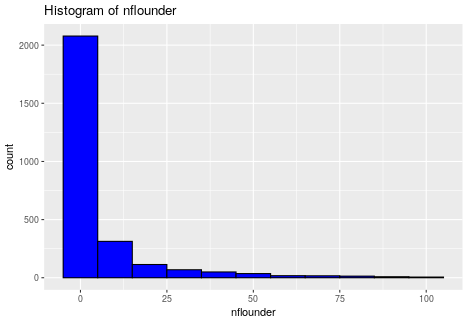
\includegraphics[keepaspectratio]{figure/unnamed-chunk-5-1.png}}
See how many values fall in each category:

\begin{Shaded}
\begin{Highlighting}[]
\CommentTok{\# Define the bin width}
\NormalTok{bin\_width }\OtherTok{\textless{}{-}} \DecValTok{10}

\CommentTok{\# Define the breaks for the bins}
\NormalTok{breaks }\OtherTok{\textless{}{-}} \FunctionTok{seq}\NormalTok{(}\FunctionTok{min}\NormalTok{(df}\SpecialCharTok{$}\NormalTok{nflounder), }\FunctionTok{max}\NormalTok{(df}\SpecialCharTok{$}\NormalTok{nflounder), }\AttributeTok{by =}\NormalTok{ bin\_width)}

\CommentTok{\# Divide the data into bins}
\NormalTok{bins }\OtherTok{\textless{}{-}} \FunctionTok{cut}\NormalTok{(df}\SpecialCharTok{$}\NormalTok{nflounder, }\AttributeTok{breaks =}\NormalTok{ breaks, }\AttributeTok{include.lowest =} \ConstantTok{TRUE}\NormalTok{, }\AttributeTok{right =} \ConstantTok{FALSE}\NormalTok{)}

\CommentTok{\# Count the number of values in each bin}
\NormalTok{bin\_counts }\OtherTok{\textless{}{-}} \FunctionTok{table}\NormalTok{(bins)}

\CommentTok{\# Print the bin counts}
\FunctionTok{print}\NormalTok{(bin\_counts)}
\end{Highlighting}
\end{Shaded}

\begin{verbatim}
## bins
##    [0,10)   [10,20)   [20,30)   [30,40)   [40,50)   [50,60)   [60,70)   [70,80) 
##      2245       205        94        57        44        20        19        16 
##   [80,90)  [90,100) [100,110) [110,120) [120,130) [130,140) [140,150) [150,160) 
##        10        13         7         5         1         2         2         3 
## [160,170) [170,180) [180,190) [190,200) [200,210) [210,220) [220,230) [230,240) 
##         2         1         0         0         2         1         4         0 
## [240,250) [250,260) [260,270) [270,280) [280,290) [290,300) [300,310) [310,320) 
##         0         1         0         1         2         0         1         0 
## [320,330) [330,340) [340,350) [350,360) [360,370) [370,380) [380,390) [390,400) 
##         1         1         0         0         0         0         0         0 
## [400,410) [410,420) [420,430] 
##         0         2         0
\end{verbatim}

Lets truncate values above 100 for modelling convenience.

\begin{Shaded}
\begin{Highlighting}[]
\NormalTok{original\_nrow }\OtherTok{\textless{}{-}} \FunctionTok{nrow}\NormalTok{(df)}
\NormalTok{df }\OtherTok{\textless{}{-}} \FunctionTok{subset}\NormalTok{(df, nflounder }\SpecialCharTok{\textless{}=} \DecValTok{100}\NormalTok{)}
\NormalTok{removed\_nrow }\OtherTok{\textless{}{-}}\NormalTok{ original\_nrow}\SpecialCharTok{{-}}\FunctionTok{nrow}\NormalTok{(df)}
\NormalTok{conditional\_var }\OtherTok{\textless{}{-}} \FunctionTok{var}\NormalTok{(df}\SpecialCharTok{$}\NormalTok{nflounder, }\AttributeTok{na.rm=}\ConstantTok{TRUE}\NormalTok{)}
\NormalTok{conditional\_mean }\OtherTok{\textless{}{-}} \FunctionTok{mean}\NormalTok{(df}\SpecialCharTok{$}\NormalTok{nflounder, }\AttributeTok{na.rm=}\ConstantTok{TRUE}\NormalTok{)}
\end{Highlighting}
\end{Shaded}

We removed 39 from 2763. Let's visualise distribution of nflounder
again.

\begin{Shaded}
\begin{Highlighting}[]
\FunctionTok{ggplot}\NormalTok{(df, }\FunctionTok{aes}\NormalTok{(nflounder)) }\SpecialCharTok{+} 
  \FunctionTok{geom\_histogram}\NormalTok{(}\AttributeTok{binwidth =} \DecValTok{10}\NormalTok{, }\AttributeTok{fill =} \StringTok{"blue"}\NormalTok{, }\AttributeTok{color =} \StringTok{"black"}\NormalTok{) }\SpecialCharTok{+}
  \FunctionTok{labs}\NormalTok{(}\AttributeTok{title =} \StringTok{"Histogram of nflounder"}\NormalTok{, }\AttributeTok{x =} \StringTok{"nflounder"}\NormalTok{)}
\end{Highlighting}
\end{Shaded}

\pandocbounded{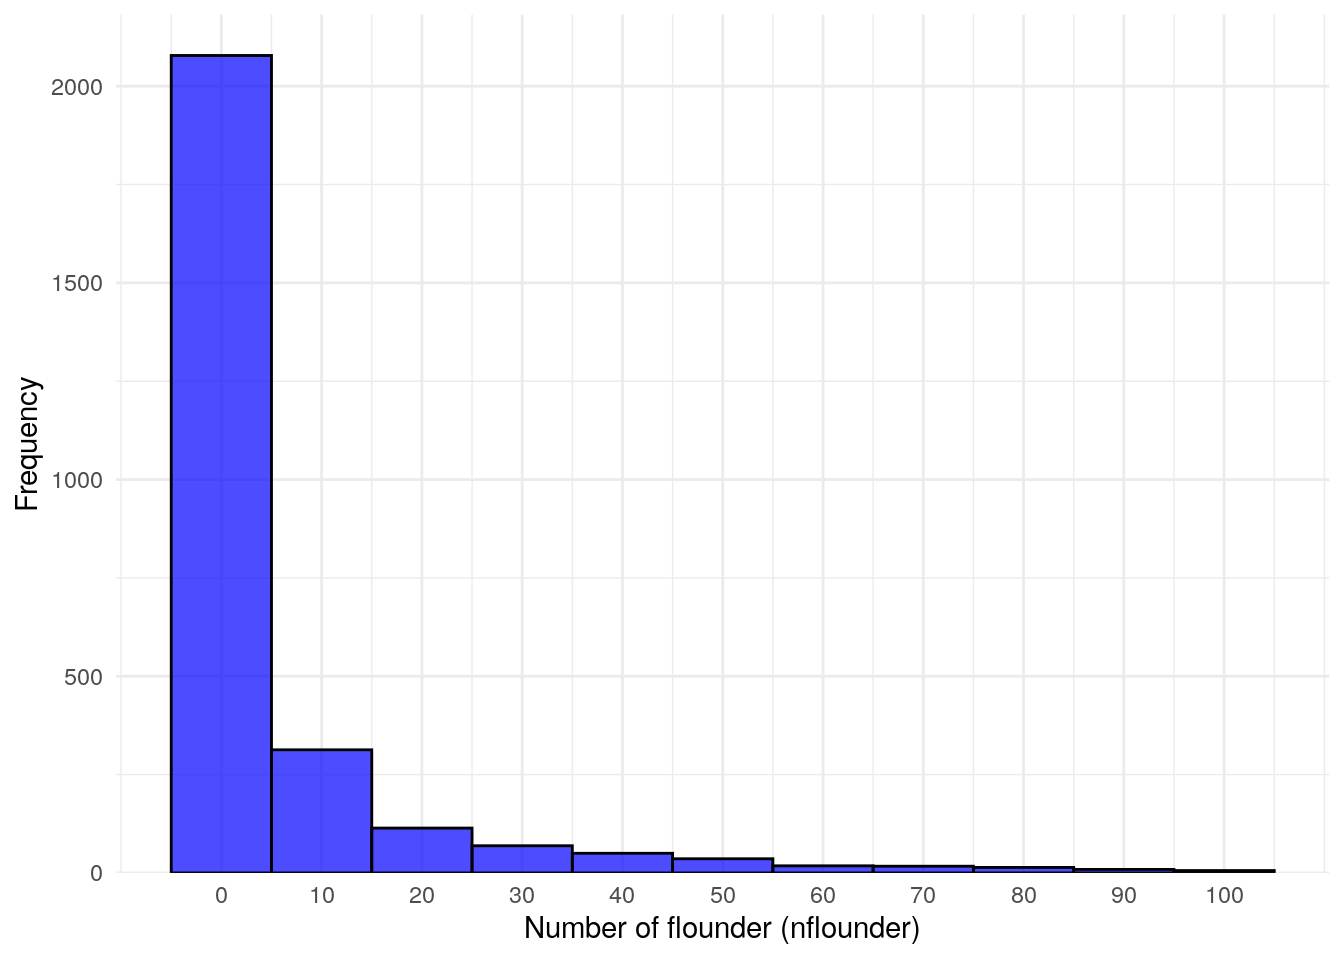
\includegraphics[keepaspectratio]{figure/unnamed-chunk-8-1.png}}
As we can see data is still highly overdispersed, the conditional
variance (208.0536609) exceeds the conditional mean (6.5179883). In
situations like this negative binomial is an appropriate distribution to
use.

\begin{Shaded}
\begin{Highlighting}[]
\FunctionTok{ggplot}\NormalTok{(df, }\FunctionTok{aes}\NormalTok{(}\AttributeTok{x =} \FunctionTok{factor}\NormalTok{(year), }\AttributeTok{y =}\NormalTok{ nflounder)) }\SpecialCharTok{+}
  \FunctionTok{geom\_boxplot}\NormalTok{() }\SpecialCharTok{+}
  \CommentTok{\# scale\_y\_log10() +}
  \FunctionTok{labs}\NormalTok{(}\AttributeTok{x =} \StringTok{"year"}\NormalTok{, }\AttributeTok{y =} \StringTok{"nflounder"}\NormalTok{, }\AttributeTok{title =} \StringTok{"nflounder vs year"}\NormalTok{)}
\end{Highlighting}
\end{Shaded}

\pandocbounded{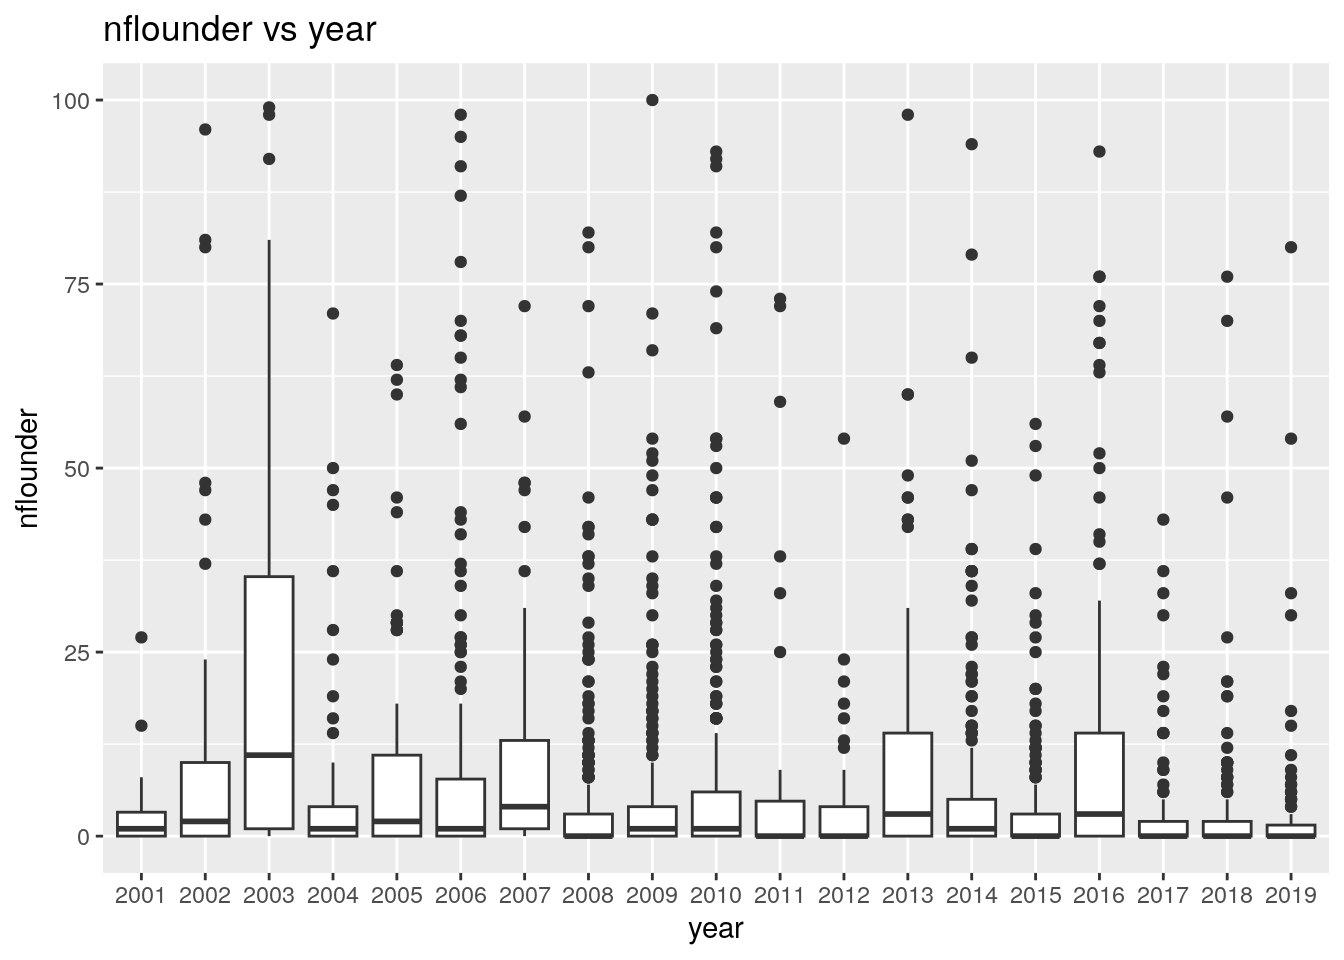
\includegraphics[keepaspectratio]{figure/unnamed-chunk-9-1.png}}

\subsection{Correlation analysis}\label{correlation-analysis}

\begin{Shaded}
\begin{Highlighting}[]
\NormalTok{df\_numeric }\OtherTok{\textless{}{-}}\NormalTok{ df[}\FunctionTok{sapply}\NormalTok{(df, is.numeric)]}
\NormalTok{cor\_matrix }\OtherTok{\textless{}{-}} \FunctionTok{cor}\NormalTok{(df\_numeric, }\AttributeTok{use =} \StringTok{"complete.obs"}\NormalTok{)}
\FunctionTok{print}\NormalTok{(cor\_matrix)}
\end{Highlighting}
\end{Shaded}

\begin{verbatim}
##                     year           lat        long    distshore        trawl
## year         1.000000000  0.0049817860 -0.06511398  0.088010356 -0.119769828
## lat          0.004981786  1.0000000000  0.04506691 -0.005444478  0.093568489
## long        -0.065113977  0.0450669064  1.00000000 -0.224120769  0.043158598
## distshore    0.088010356 -0.0054444775 -0.22412077  1.000000000  0.144581861
## trawl       -0.119769828  0.0935684891  0.04315860  0.144581861  1.000000000
## area         0.067678064 -0.0007925651 -0.10255599  0.164351090 -0.028732391
## chlorophyll  0.070847279 -0.0322708516  0.14170391  0.020114161  0.003544562
## tempavg      0.093554648 -0.2230929909 -0.04791776  0.084518093 -0.022062488
## tempstdev   -0.156715923 -0.0234881935 -0.05046801  0.096050784  0.025851643
## sal         -0.204827187  0.3989884868 -0.12004630 -0.050253948  0.029244586
## bod         -0.125186675 -0.3154381712  0.25662766 -0.113689564  0.051555411
## nh3         -0.269058242 -0.1454581609  0.24194535 -0.078002487  0.013807491
## po4         -0.159703341 -0.1719509276  0.50093553  0.038484470 -0.036196786
## depth        0.118780600 -0.3806972918  0.20077301  0.045172606 -0.005677570
## nflounder   -0.096151776 -0.1291115877  0.18078237 -0.132022226 -0.002051093
##                      area  chlorophyll     tempavg   tempstdev         sal
## year         0.0676780642  0.070847279  0.09355465 -0.15671592 -0.20482719
## lat         -0.0007925651 -0.032270852 -0.22309299 -0.02348819  0.39898849
## long        -0.1025559916  0.141703905 -0.04791776 -0.05046801 -0.12004630
## distshore    0.1643510905  0.020114161  0.08451809  0.09605078 -0.05025395
## trawl       -0.0287323909  0.003544562 -0.02206249  0.02585164  0.02924459
## area         1.0000000000 -0.007407639 -0.07788099  0.11644657 -0.09950945
## chlorophyll -0.0074076388  1.000000000  0.18577262  0.10878705  0.03726607
## tempavg     -0.0778809900  0.185772616  1.00000000  0.20038897 -0.19076514
## tempstdev    0.1164465703  0.108787049  0.20038897  1.00000000 -0.04111293
## sal         -0.0995094464  0.037266065 -0.19076514 -0.04111293  1.00000000
## bod         -0.1491648863  0.148704747 -0.05496218  0.08648001  0.12076372
## nh3         -0.0667732092 -0.026391337 -0.07254021  0.02594419  0.41822587
## po4          0.1422456757 -0.101320955 -0.02263963  0.05345896 -0.14777738
## depth        0.1227755778 -0.028296778  0.13414873  0.01176289 -0.64814422
## nflounder   -0.0897024377  0.015470871  0.07377867  0.04200609 -0.19505829
##                     bod         nh3         po4       depth    nflounder
## year        -0.12518667 -0.26905824 -0.15970334  0.11878060 -0.096151776
## lat         -0.31543817 -0.14545816 -0.17195093 -0.38069729 -0.129111588
## long         0.25662766  0.24194535  0.50093553  0.20077301  0.180782366
## distshore   -0.11368956 -0.07800249  0.03848447  0.04517261 -0.132022226
## trawl        0.05155541  0.01380749 -0.03619679 -0.00567757 -0.002051093
## area        -0.14916489 -0.06677321  0.14224568  0.12277558 -0.089702438
## chlorophyll  0.14870475 -0.02639134 -0.10132096 -0.02829678  0.015470871
## tempavg     -0.05496218 -0.07254021 -0.02263963  0.13414873  0.073778667
## tempstdev    0.08648001  0.02594419  0.05345896  0.01176289  0.042006088
## sal          0.12076372  0.41822587 -0.14777738 -0.64814422 -0.195058290
## bod          1.00000000  0.42517649  0.35803600 -0.12377171  0.085604235
## nh3          0.42517649  1.00000000  0.48816749 -0.37503797 -0.015704750
## po4          0.35803600  0.48816749  1.00000000  0.18052167  0.059434892
## depth       -0.12377171 -0.37503797  0.18052167  1.00000000  0.113621304
## nflounder    0.08560423 -0.01570475  0.05943489  0.11362130  1.000000000
\end{verbatim}

\begin{Shaded}
\begin{Highlighting}[]
\CommentTok{\# Melt the correlation matrix into a long format}
\NormalTok{cor\_matrix\_melted }\OtherTok{\textless{}{-}} \FunctionTok{melt}\NormalTok{(cor\_matrix)}

\CommentTok{\# Plot the heatmap using ggplot2}
\FunctionTok{ggplot}\NormalTok{(}\AttributeTok{data =}\NormalTok{ cor\_matrix\_melted, }\FunctionTok{aes}\NormalTok{(}\AttributeTok{x=}\NormalTok{Var1, }\AttributeTok{y=}\NormalTok{Var2, }\AttributeTok{fill=}\NormalTok{value)) }\SpecialCharTok{+}
  \FunctionTok{geom\_tile}\NormalTok{() }\SpecialCharTok{+}
  \FunctionTok{scale\_fill\_gradient2}\NormalTok{(}\AttributeTok{low =} \StringTok{"blue"}\NormalTok{, }\AttributeTok{high =} \StringTok{"red"}\NormalTok{, }\AttributeTok{mid =} \StringTok{"white"}\NormalTok{, }
                       \AttributeTok{midpoint =} \DecValTok{0}\NormalTok{, }\AttributeTok{limit =} \FunctionTok{c}\NormalTok{(}\SpecialCharTok{{-}}\DecValTok{1}\NormalTok{,}\DecValTok{1}\NormalTok{), }\AttributeTok{space =} \StringTok{"Lab"}\NormalTok{, }
                       \AttributeTok{name=}\StringTok{"Pearson}\SpecialCharTok{\textbackslash{}n}\StringTok{Correlation"}\NormalTok{) }\SpecialCharTok{+}
  \FunctionTok{theme\_minimal}\NormalTok{() }\SpecialCharTok{+} 
  \FunctionTok{theme}\NormalTok{(}\AttributeTok{axis.text.x =} \FunctionTok{element\_text}\NormalTok{(}\AttributeTok{angle =} \DecValTok{90}\NormalTok{, }\AttributeTok{vjust =} \DecValTok{1}\NormalTok{, }
                                   \AttributeTok{size =} \DecValTok{9}\NormalTok{, }\AttributeTok{hjust =} \DecValTok{1}\NormalTok{), }
        \AttributeTok{axis.title.x =} \FunctionTok{element\_blank}\NormalTok{(), }\CommentTok{\# Remove x{-}axis title}
        \AttributeTok{axis.title.y =} \FunctionTok{element\_blank}\NormalTok{(),) }\SpecialCharTok{+}
  
  \FunctionTok{coord\_fixed}\NormalTok{()}
\end{Highlighting}
\end{Shaded}

\pandocbounded{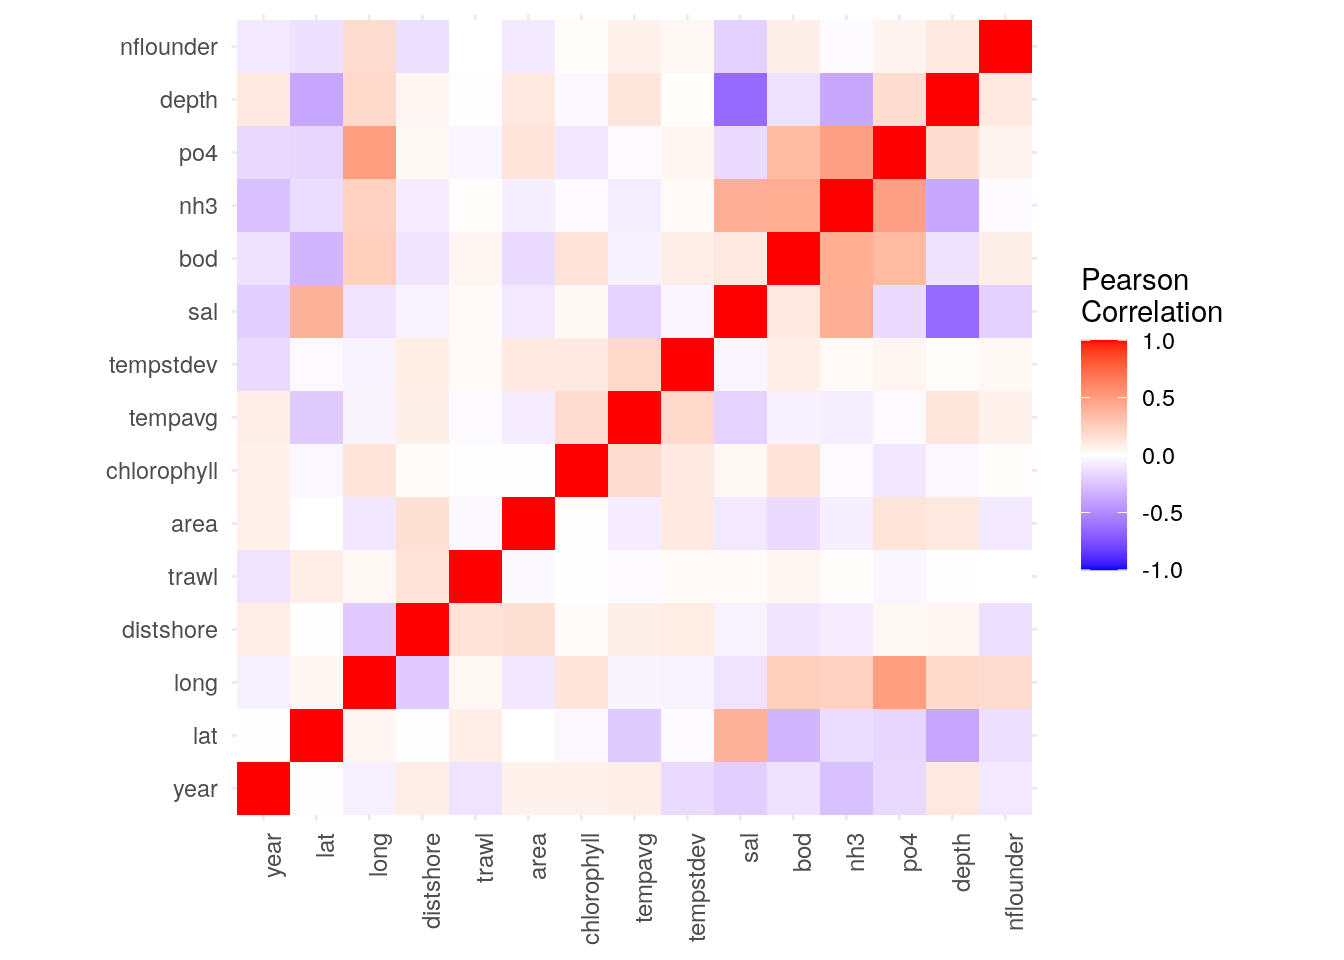
\includegraphics[keepaspectratio]{figure/unnamed-chunk-10-1.png}}

\subsection{Zero-inflation}\label{zero-inflation}

\begin{Shaded}
\begin{Highlighting}[]
\CommentTok{\# Calculate the proportion of values that are 0}
\NormalTok{zero\_proportion }\OtherTok{\textless{}{-}} \FunctionTok{mean}\NormalTok{(df}\SpecialCharTok{$}\NormalTok{nflounder }\SpecialCharTok{==} \DecValTok{0}\NormalTok{)}
\end{Highlighting}
\end{Shaded}

The proportion of zeros in nflounder is 0.4533774.

\subsection{Scale variables}\label{scale-variables}

We shall scale some of the variables to avoid numerical overflow.

\begin{Shaded}
\begin{Highlighting}[]
\NormalTok{var\_to\_scale }\OtherTok{\textless{}{-}} \FunctionTok{c}\NormalTok{(}\StringTok{"distshore"}\NormalTok{, }\StringTok{"area"}\NormalTok{,}\StringTok{"chlorophyll"}\NormalTok{)}
\NormalTok{df[, var\_to\_scale] }\OtherTok{\textless{}{-}} \FunctionTok{scale}\NormalTok{(df[, var\_to\_scale])}
\end{Highlighting}
\end{Shaded}

Consider discarding some of the variables, e.g.~\texttt{trawl}, in which
the proportion of 0's (should be NA's?) 0.8509545.

\begin{Shaded}
\begin{Highlighting}[]
\NormalTok{df }\OtherTok{\textless{}{-}} \FunctionTok{subset}\NormalTok{(df, }\AttributeTok{select =} \SpecialCharTok{{-}}\NormalTok{trawl)}
\end{Highlighting}
\end{Shaded}

\section{Data modelling}\label{data-modelling}

\subsection{Negative binomial GLM}\label{negative-binomial-glm}

We fit a negative binomial generalized linear model with log link to the
full dataset, excluding site, trawl and net for the moment. This model
is useful for count data that exhibit overdispersion (the var exceeds
the mean). Let \(Y_i\) denote the count response variable for the
\(i\)-th observation. The negative binomial distribution for \(Y_i\) is
parameterised by the mean \(\lambda_i\) and the dispersion parameter
\(\theta\):

\[
Y_i \sim \text{NB}(\lambda_i, \theta)
\]

where the probability mass function is given by:

\[
P(Y_i = k) = \binom{k + \theta - 1}{k} \left( \frac{\theta}{\theta + \lambda_i} \right)^\theta \left( \frac{\lambda_i}{\theta + \lambda_i} \right)^k, \quad k = 0, 1, 2, \ldots
\]

\subsubsection{Log Link Function}\label{log-link-function}

The relationship between the mean \(\lambda_i\) and the explanatory
variables \(\mathbf{X}_i\) is modeled using a log link function:

\[
\log(\lambda_i) = \mathbf{X}_i \boldsymbol{\beta}
\]

where:

\begin{itemize}
    \item \( \lambda_i \) is the expected count for the \( i \)-th observation.
    \item \( \mathbf{X}_i \) is a vector of explanatory variables for the \( i \)-th observation.
    \item \( \boldsymbol{\beta} \) is a vector of coefficients to be estimated.
\end{itemize}

\subsubsection{Linear Predictor}\label{linear-predictor}

The linear predictor is given: \[
\eta_i = \mathbf{X}_i \boldsymbol{\beta}
\] where \(\eta_i = \log(\lambda_i)\). Therefore, the model can be
rewritten as:

\[
\lambda_i = \exp(\mathbf{X}_i \boldsymbol{\beta})
\]

\begin{Shaded}
\begin{Highlighting}[]
\NormalTok{m.glmm.fixed }\OtherTok{\textless{}{-}} \FunctionTok{glmmTMB}\NormalTok{(}
\NormalTok{  nflounder }\SpecialCharTok{\textasciitilde{}}\NormalTok{ year }\SpecialCharTok{+}\NormalTok{ lat }\SpecialCharTok{+}\NormalTok{ long }\SpecialCharTok{+}\NormalTok{ distshore }\SpecialCharTok{+}\NormalTok{ area }\SpecialCharTok{+}\NormalTok{ chlorophyll }\SpecialCharTok{+}\NormalTok{ tempavg }\SpecialCharTok{+}\NormalTok{ tempstdev }\SpecialCharTok{+}\NormalTok{ sal }\SpecialCharTok{+}\NormalTok{ bod }\SpecialCharTok{+}\NormalTok{ nh3 }\SpecialCharTok{+}\NormalTok{ po4 }\SpecialCharTok{+}\NormalTok{ depth, }
  \AttributeTok{data =}\NormalTok{ df, }
  \AttributeTok{family =} \FunctionTok{nbinom2}\NormalTok{()}
\NormalTok{)}
\FunctionTok{summary}\NormalTok{(m.glmm.fixed)}
\end{Highlighting}
\end{Shaded}

\begin{verbatim}
##  Family: nbinom2  ( log )
## Formula:          
## nflounder ~ year + lat + long + distshore + area + chlorophyll +  
##     tempavg + tempstdev + sal + bod + nh3 + po4 + depth
## Data: df
## 
##      AIC      BIC   logLik deviance df.resid 
##  12986.0  13074.7  -6478.0  12956.0     2709 
## 
## 
## Dispersion parameter for nbinom2 family (): 0.275 
## 
## Conditional model:
##               Estimate Std. Error z value Pr(>|z|)    
## (Intercept) 142.085983  18.135502   7.835 4.70e-15 ***
## year         -0.067561   0.008911  -7.582 3.42e-14 ***
## lat          -0.031889   0.069301  -0.460  0.64541    
## long          0.264338   0.045712   5.783 7.35e-09 ***
## distshore    -0.337031   0.039239  -8.589  < 2e-16 ***
## area         -0.086590   0.034720  -2.494  0.01263 *  
## chlorophyll  -0.049502   0.043955  -1.126  0.26008    
## tempavg       0.041370   0.024032   1.721  0.08516 .  
## tempstdev     0.071309   0.031546   2.260  0.02379 *  
## sal          -0.095546   0.010504  -9.096  < 2e-16 ***
## bod           0.075791   0.079467   0.954  0.34021    
## nh3           4.690307   2.031163   2.309  0.02093 *  
## po4          -0.009337   0.004179  -2.234  0.02546 *  
## depth        -0.078342   0.028648  -2.735  0.00624 ** 
## ---
## Signif. codes:  0 '***' 0.001 '**' 0.01 '*' 0.05 '.' 0.1 ' ' 1
\end{verbatim}

\subsection{Negative Binomial GLMM}\label{negative-binomial-glmm}

Lets add random effect of site and net to the best model. This is an
additional term that accounts for unobserved heterogeneity in the data.
Random effects are used when data are collected in clusters or groups,
and there may be variability between these groups that is not captured
by the observed explanatory variables.

\subsubsection{Random Effects}\label{random-effects}

The random effects \(u_j\) are assumed to follow a normal distribution
with mean zero and variance \(\sigma^2_u\):

\[
u_j \sim \mathcal{N}(0, \sigma^2_u)
\]

\subsubsection{Linear Predictor}\label{linear-predictor-1}

The linear predictor is given by:

\[
\eta_{ij} = \mathbf{X}_{ij} \boldsymbol{\beta} + u_j
\]

where \(\eta_{ij} = \log(\lambda_{ij})\). Therefore, the model can be
rewritten as:

\[
\lambda_{ij} = \exp(\mathbf{X}_{ij} \boldsymbol{\beta} + u_j)
\]

\begin{Shaded}
\begin{Highlighting}[]
\CommentTok{\# a model of crossed random effects (site and net)}
\NormalTok{m.glmm.random1 }\OtherTok{\textless{}{-}} \FunctionTok{glmmTMB}\NormalTok{(}
\NormalTok{  nflounder }\SpecialCharTok{\textasciitilde{}}\NormalTok{ year }\SpecialCharTok{+}\NormalTok{ lat }\SpecialCharTok{+}\NormalTok{ long }\SpecialCharTok{+}\NormalTok{ distshore }\SpecialCharTok{+}\NormalTok{ area }\SpecialCharTok{+}\NormalTok{ chlorophyll }\SpecialCharTok{+}\NormalTok{ tempavg }\SpecialCharTok{+}\NormalTok{ tempstdev }\SpecialCharTok{+}\NormalTok{ sal }\SpecialCharTok{+}\NormalTok{ bod }\SpecialCharTok{+}\NormalTok{ nh3 }\SpecialCharTok{+}\NormalTok{ po4 }\SpecialCharTok{+}\NormalTok{ depth }\SpecialCharTok{+}\NormalTok{ (}\DecValTok{1} \SpecialCharTok{|}\NormalTok{ site) }\SpecialCharTok{+}\NormalTok{ (}\DecValTok{1} \SpecialCharTok{|}\NormalTok{ net), }
  \AttributeTok{data =}\NormalTok{ df, }
  \AttributeTok{family =} \FunctionTok{nbinom2}\NormalTok{()}
\NormalTok{)}
\FunctionTok{summary}\NormalTok{(m.glmm.random1)}
\end{Highlighting}
\end{Shaded}

\begin{verbatim}
##  Family: nbinom2  ( log )
## Formula:          
## nflounder ~ year + lat + long + distshore + area + chlorophyll +  
##     tempavg + tempstdev + sal + bod + nh3 + po4 + depth + (1 |  
##     site) + (1 | net)
## Data: df
## 
##      AIC      BIC   logLik deviance df.resid 
##  12633.4  12733.9  -6299.7  12599.4     2707 
## 
## Random effects:
## 
## Conditional model:
##  Groups Name        Variance  Std.Dev. 
##  site   (Intercept) 1.086e+00 1.0421893
##  net    (Intercept) 1.813e-08 0.0001346
## Number of obs: 2724, groups:  site, 74; net, 3
## 
## Dispersion parameter for nbinom2 family (): 0.356 
## 
## Conditional model:
##               Estimate Std. Error z value Pr(>|z|)    
## (Intercept) 146.856572  22.283365   6.590 4.39e-11 ***
## year         -0.079193   0.009943  -7.965 1.66e-15 ***
## lat           0.297084   0.177035   1.678   0.0933 .  
## long          0.268307   0.133346   2.012   0.0442 *  
## distshore    -0.340952   0.052580  -6.484 8.91e-11 ***
## area          0.010225   0.045513   0.225   0.8222    
## chlorophyll  -0.117903   0.045901  -2.569   0.0102 *  
## tempavg       0.054199   0.025686   2.110   0.0349 *  
## tempstdev     0.043631   0.036127   1.208   0.2272    
## sal          -0.092916   0.021349  -4.352 1.35e-05 ***
## bod           0.462236   0.242099   1.909   0.0562 .  
## nh3          -4.194333   4.324354  -0.970   0.3321    
## po4           0.014944   0.011991   1.246   0.2127    
## depth        -0.083901   0.084408  -0.994   0.3202    
## ---
## Signif. codes:  0 '***' 0.001 '**' 0.01 '*' 0.05 '.' 0.1 ' ' 1
\end{verbatim}

\begin{Shaded}
\begin{Highlighting}[]
\CommentTok{\# alternatively we consider a model of nested random effects (net within a site since nets were reused across sites)}

\NormalTok{m.glmm.random2 }\OtherTok{\textless{}{-}} \FunctionTok{glmmTMB}\NormalTok{(}
\NormalTok{    nflounder }\SpecialCharTok{\textasciitilde{}}\NormalTok{ year }\SpecialCharTok{+}\NormalTok{ lat }\SpecialCharTok{+}\NormalTok{ long }\SpecialCharTok{+}\NormalTok{ distshore }\SpecialCharTok{+}\NormalTok{ area }\SpecialCharTok{+}\NormalTok{ chlorophyll }\SpecialCharTok{+}\NormalTok{ tempavg }\SpecialCharTok{+}\NormalTok{ tempstdev }\SpecialCharTok{+}\NormalTok{ sal }\SpecialCharTok{+}\NormalTok{ bod }\SpecialCharTok{+}\NormalTok{ nh3 }\SpecialCharTok{+}\NormalTok{ po4 }\SpecialCharTok{+}\NormalTok{ depth }\SpecialCharTok{+}\NormalTok{ (}\DecValTok{1} \SpecialCharTok{|}\NormalTok{ site}\SpecialCharTok{/}\NormalTok{net), }
    \AttributeTok{data =}\NormalTok{ df, }
    \AttributeTok{family =} \FunctionTok{nbinom2}\NormalTok{()}
\NormalTok{)}
\FunctionTok{summary}\NormalTok{(m.glmm.random2)}
\end{Highlighting}
\end{Shaded}

\begin{verbatim}
##  Family: nbinom2  ( log )
## Formula:          
## nflounder ~ year + lat + long + distshore + area + chlorophyll +  
##     tempavg + tempstdev + sal + bod + nh3 + po4 + depth + (1 |      site/net)
## Data: df
## 
##      AIC      BIC   logLik deviance df.resid 
##  12620.4  12720.9  -6293.2  12586.4     2707 
## 
## Random effects:
## 
## Conditional model:
##  Groups   Name        Variance Std.Dev.
##  net:site (Intercept) 0.1387   0.3724  
##  site     (Intercept) 0.9891   0.9945  
## Number of obs: 2724, groups:  net:site, 191; site, 74
## 
## Dispersion parameter for nbinom2 family (): 0.367 
## 
## Conditional model:
##               Estimate Std. Error z value Pr(>|z|)    
## (Intercept) 143.642489  22.690961   6.330 2.45e-10 ***
## year         -0.077686   0.010172  -7.637 2.22e-14 ***
## lat           0.302926   0.174863   1.732   0.0832 .  
## long          0.278606   0.131623   2.117   0.0343 *  
## distshore    -0.319119   0.053400  -5.976 2.29e-09 ***
## area         -0.007699   0.046434  -0.166   0.8683    
## chlorophyll  -0.098694   0.046527  -2.121   0.0339 *  
## tempavg       0.049323   0.025896   1.905   0.0568 .  
## tempstdev     0.051795   0.036576   1.416   0.1567    
## sal          -0.096830   0.021197  -4.568 4.92e-06 ***
## bod           0.433694   0.238992   1.815   0.0696 .  
## nh3          -3.737041   4.264675  -0.876   0.3809    
## po4           0.015004   0.011836   1.268   0.2049    
## depth        -0.075507   0.083328  -0.906   0.3649    
## ---
## Signif. codes:  0 '***' 0.001 '**' 0.01 '*' 0.05 '.' 0.1 ' ' 1
\end{verbatim}

\begin{Shaded}
\begin{Highlighting}[]
\CommentTok{\# year|site for a model with random variation in slopes through years across sites}
\NormalTok{m.glmm.random3 }\OtherTok{\textless{}{-}} \FunctionTok{glmmTMB}\NormalTok{(}
\NormalTok{    nflounder }\SpecialCharTok{\textasciitilde{}}\NormalTok{ lat }\SpecialCharTok{+}\NormalTok{ long }\SpecialCharTok{+}\NormalTok{ distshore }\SpecialCharTok{+}\NormalTok{ area }\SpecialCharTok{+}\NormalTok{ chlorophyll }\SpecialCharTok{+}\NormalTok{ tempavg }\SpecialCharTok{+}\NormalTok{ tempstdev }\SpecialCharTok{+}\NormalTok{ sal }\SpecialCharTok{+}\NormalTok{ bod }\SpecialCharTok{+}\NormalTok{ nh3 }\SpecialCharTok{+}\NormalTok{ po4 }\SpecialCharTok{+}\NormalTok{ depth }\SpecialCharTok{+}\NormalTok{ (year }\SpecialCharTok{|}\NormalTok{ site) }\SpecialCharTok{+}\NormalTok{ (}\DecValTok{1}\SpecialCharTok{|}\NormalTok{net), }
    \AttributeTok{data =}\NormalTok{ df, }
    \AttributeTok{family =} \FunctionTok{nbinom2}\NormalTok{()}
\NormalTok{)}
\FunctionTok{summary}\NormalTok{(m.glmm.random3)}
\end{Highlighting}
\end{Shaded}

\begin{verbatim}
##  Family: nbinom2  ( log )
## Formula:          
## nflounder ~ lat + long + distshore + area + chlorophyll + tempavg +  
##     tempstdev + sal + bod + nh3 + po4 + depth + (year | site) +      (1 | net)
## Data: df
## 
##      AIC      BIC   logLik deviance df.resid 
##  12635.0  12741.3  -6299.5  12599.0     2706 
## 
## Random effects:
## 
## Conditional model:
##  Groups Name        Variance  Std.Dev.  Corr  
##  site   (Intercept) 8.495e+04 2.915e+02       
##         year        2.104e-02 1.451e-01 -1.00 
##  net    (Intercept) 4.652e-08 2.157e-04       
## Number of obs: 2724, groups:  site, 74; net, 3
## 
## Dispersion parameter for nbinom2 family (): 0.368 
## 
## Conditional model:
##              Estimate Std. Error z value Pr(>|z|)    
## (Intercept) -17.23222   10.24436  -1.682   0.0925 .  
## lat           0.38671    0.18179   2.127   0.0334 *  
## long          0.20767    0.13643   1.522   0.1280    
## distshore    -0.34926    0.05252  -6.650 2.94e-11 ***
## area          0.02208    0.05015   0.440   0.6597    
## chlorophyll  -0.10360    0.04803  -2.157   0.0310 *  
## tempavg       0.02584    0.02631   0.982   0.3260    
## tempstdev     0.04094    0.03928   1.042   0.2973    
## sal          -0.09750    0.02211  -4.409 1.04e-05 ***
## bod           0.48615    0.25131   1.934   0.0531 .  
## nh3          -4.83216    4.37859  -1.104   0.2698    
## po4           0.02072    0.01246   1.663   0.0963 .  
## depth        -0.08201    0.08681  -0.945   0.3449    
## ---
## Signif. codes:  0 '***' 0.001 '**' 0.01 '*' 0.05 '.' 0.1 ' ' 1
\end{verbatim}

Lets compare fixed and random effect models.

\begin{Shaded}
\begin{Highlighting}[]
\FunctionTok{anova}\NormalTok{(m.glmm.fixed, m.glmm.random1, m.glmm.random2, m.glmm.random3)}
\end{Highlighting}
\end{Shaded}

\begin{verbatim}
## Data: df
## Models:
## m.glmm.fixed: nflounder ~ year + lat + long + distshore + area + chlorophyll + , zi=~0, disp=~1
## m.glmm.fixed:     tempavg + tempstdev + sal + bod + nh3 + po4 + depth, zi=~0, disp=~1
## m.glmm.random1: nflounder ~ year + lat + long + distshore + area + chlorophyll + , zi=~0, disp=~1
## m.glmm.random1:     tempavg + tempstdev + sal + bod + nh3 + po4 + depth + (1 | , zi=~0, disp=~1
## m.glmm.random1:     site) + (1 | net), zi=~0, disp=~1
## m.glmm.random2: nflounder ~ year + lat + long + distshore + area + chlorophyll + , zi=~0, disp=~1
## m.glmm.random2:     tempavg + tempstdev + sal + bod + nh3 + po4 + depth + (1 | , zi=~0, disp=~1
## m.glmm.random2:     site/net), zi=~0, disp=~1
## m.glmm.random3: nflounder ~ lat + long + distshore + area + chlorophyll + tempavg + , zi=~0, disp=~1
## m.glmm.random3:     tempstdev + sal + bod + nh3 + po4 + depth + (year | site) + , zi=~0, disp=~1
## m.glmm.random3:     (1 | net), zi=~0, disp=~1
##                Df   AIC   BIC  logLik deviance   Chisq Chi Df Pr(>Chisq)    
## m.glmm.fixed   15 12986 13075 -6478.0    12956                              
## m.glmm.random1 17 12633 12734 -6299.7    12599 356.660      2     <2e-16 ***
## m.glmm.random2 17 12620 12721 -6293.2    12586  12.963      0     <2e-16 ***
## m.glmm.random3 18 12635 12741 -6299.5    12599   0.000      1          1    
## ---
## Signif. codes:  0 '***' 0.001 '**' 0.01 '*' 0.05 '.' 0.1 ' ' 1
\end{verbatim}

We choose the model with lowest AIC which is \texttt{m.glmm.random2}, a
model of nested random effects (net within a site).

\subsection{Zero-inflated poisson
GLMM}\label{zero-inflated-poisson-glmm}

Now lets try a zero-inflated Poisson model with a single zero inflation
parameter applying to all observations using ziformula\textasciitilde1.

\begin{Shaded}
\begin{Highlighting}[]
\NormalTok{m.glmm.random.zero }\OtherTok{\textless{}{-}} \FunctionTok{glmmTMB}\NormalTok{(}
\NormalTok{    nflounder }\SpecialCharTok{\textasciitilde{}}\NormalTok{ year }\SpecialCharTok{+}\NormalTok{ lat }\SpecialCharTok{+}\NormalTok{ long }\SpecialCharTok{+}\NormalTok{ distshore }\SpecialCharTok{+}\NormalTok{ area }\SpecialCharTok{+}\NormalTok{ chlorophyll }\SpecialCharTok{+}\NormalTok{ tempavg }\SpecialCharTok{+}\NormalTok{ tempstdev }\SpecialCharTok{+}\NormalTok{ sal }\SpecialCharTok{+}\NormalTok{ bod }\SpecialCharTok{+}\NormalTok{ nh3 }\SpecialCharTok{+}\NormalTok{ po4 }\SpecialCharTok{+}\NormalTok{ depth }\SpecialCharTok{+}\NormalTok{ (}\DecValTok{1} \SpecialCharTok{|}\NormalTok{ site}\SpecialCharTok{/}\NormalTok{net), }
    \AttributeTok{data =}\NormalTok{ df, }
    \AttributeTok{ziformula=}\SpecialCharTok{\textasciitilde{}}\DecValTok{1}\NormalTok{,}
    \AttributeTok{family =} \FunctionTok{poisson}\NormalTok{()}
\NormalTok{)}
\end{Highlighting}
\end{Shaded}

\begin{verbatim}
## Warning in (function (start, objective, gradient = NULL, hessian = NULL, :
## NA/NaN function evaluation
## Warning in (function (start, objective, gradient = NULL, hessian = NULL, :
## NA/NaN function evaluation
\end{verbatim}

\begin{Shaded}
\begin{Highlighting}[]
\FunctionTok{summary}\NormalTok{(m.glmm.random.zero)}
\end{Highlighting}
\end{Shaded}

\begin{verbatim}
##  Family: poisson  ( log )
## Formula:          
## nflounder ~ year + lat + long + distshore + area + chlorophyll +  
##     tempavg + tempstdev + sal + bod + nh3 + po4 + depth + (1 |      site/net)
## Zero inflation:             ~1
## Data: df
## 
##      AIC      BIC   logLik deviance df.resid 
##  26443.9  26544.3 -13204.9  26409.9     2707 
## 
## Random effects:
## 
## Conditional model:
##  Groups   Name        Variance Std.Dev.
##  net:site (Intercept)  0.5892  0.7676  
##  site     (Intercept) 28.6579  5.3533  
## Number of obs: 2724, groups:  net:site, 191; site, 74
## 
## Conditional model:
##               Estimate Std. Error z value Pr(>|z|)    
## (Intercept) -2.548e+02  1.552e+01 -16.415  < 2e-16 ***
## year        -4.676e-02  2.152e-03 -21.729  < 2e-16 ***
## lat          6.265e+00  2.798e-01  22.390  < 2e-16 ***
## long        -1.380e+00  1.405e-01  -9.820  < 2e-16 ***
## distshore   -2.792e-01  2.195e-02 -12.718  < 2e-16 ***
## area         9.999e-03  1.305e-02   0.766  0.44351    
## chlorophyll -2.942e-02  9.872e-03  -2.980  0.00288 ** 
## tempavg      4.913e-02  6.204e-03   7.918 2.40e-15 ***
## tempstdev   -1.869e-02  7.958e-03  -2.349  0.01882 *  
## sal         -1.532e-01  8.080e-02  -1.896  0.05792 .  
## bod          4.488e+00  1.013e+00   4.430 9.44e-06 ***
## nh3         -2.895e+01  1.053e+01  -2.749  0.00598 ** 
## po4          6.538e-02  5.017e-02   1.303  0.19253    
## depth        5.195e-01  3.564e-01   1.458  0.14497    
## ---
## Signif. codes:  0 '***' 0.001 '**' 0.01 '*' 0.05 '.' 0.1 ' ' 1
## 
## Zero-inflation model:
##             Estimate Std. Error z value Pr(>|z|)    
## (Intercept) -0.57605    0.04689  -12.28   <2e-16 ***
## ---
## Signif. codes:  0 '***' 0.001 '**' 0.01 '*' 0.05 '.' 0.1 ' ' 1
\end{verbatim}

This model has higher AIC, hence we prefer binomial models.

\subsection{Truncated Negative Binomial GLMM (Hurdle
Model).}\label{truncated-negative-binomial-glmm-hurdle-model.}

In contrast to zero-inflated models, hurdle models treat zero-count and
nonzero outcomes as two completely separate categories, rather than
treating the zero-count outcomes as a mixture of structural and sampling
zeros.

\begin{Shaded}
\begin{Highlighting}[]
\NormalTok{m.glmm.random2.hurdle }\OtherTok{\textless{}{-}} \FunctionTok{update}\NormalTok{ (m.glmm.random2,}
                                 \AttributeTok{data=}\NormalTok{df,}
                                 \AttributeTok{ziformula=}\SpecialCharTok{\textasciitilde{}}\NormalTok{.,}
                                 \AttributeTok{family=}\FunctionTok{truncated\_nbinom2}\NormalTok{())}
\FunctionTok{summary}\NormalTok{(m.glmm.random2.hurdle)}
\end{Highlighting}
\end{Shaded}

\begin{verbatim}
##  Family: truncated_nbinom2  ( log )
## Formula:          
## nflounder ~ year + lat + long + distshore + area + chlorophyll +  
##     tempavg + tempstdev + sal + bod + nh3 + po4 + depth + (1 |      site/net)
## Zero inflation:             ~.
## Data: df
## 
##      AIC      BIC   logLik deviance df.resid 
##  12602.9  12797.9  -6268.4  12536.9     2691 
## 
## Random effects:
## 
## Conditional model:
##  Groups   Name        Variance Std.Dev.
##  net:site (Intercept) 0.08004  0.2829  
##  site     (Intercept) 0.70242  0.8381  
## Number of obs: 2724, groups:  net:site, 191; site, 74
## 
## Zero-inflation model:
##  Groups   Name        Variance Std.Dev.
##  net:site (Intercept) 0.1106   0.3325  
##  site     (Intercept) 0.4699   0.6855  
## Number of obs: 2724, groups:  net:site, 191; site, 74
## 
## Dispersion parameter for truncated_nbinom2 family (): 0.28 
## 
## Conditional model:
##               Estimate Std. Error z value Pr(>|z|)    
## (Intercept)  1.123e+02  2.642e+01   4.252 2.12e-05 ***
## year        -6.124e-02  1.239e-02  -4.945 7.63e-07 ***
## lat          2.450e-01  1.710e-01   1.433 0.151930    
## long         8.322e-02  1.251e-01   0.665 0.505776    
## distshore   -3.746e-01  7.180e-02  -5.218 1.81e-07 ***
## area        -1.690e-02  5.471e-02  -0.309 0.757388    
## chlorophyll -6.165e-02  6.006e-02  -1.026 0.304673    
## tempavg      6.412e-02  3.245e-02   1.976 0.048186 *  
## tempstdev    4.099e-04  4.514e-02   0.009 0.992755    
## sal         -8.562e-02  2.212e-02  -3.871 0.000108 ***
## bod          2.785e-01  2.219e-01   1.255 0.209523    
## nh3         -4.264e+00  4.294e+00  -0.993 0.320633    
## po4          1.256e-02  1.109e-02   1.132 0.257518    
## depth       -8.218e-02  8.350e-02  -0.984 0.325041    
## ---
## Signif. codes:  0 '***' 0.001 '**' 0.01 '*' 0.05 '.' 0.1 ' ' 1
## 
## Zero-inflation model:
##               Estimate Std. Error z value Pr(>|z|)    
## (Intercept) -1.625e+02  2.596e+01  -6.260 3.86e-10 ***
## year         7.956e-02  1.234e-02   6.446 1.15e-10 ***
## lat         -3.740e-02  1.371e-01  -0.273 0.785028    
## long        -4.484e-01  1.057e-01  -4.243 2.21e-05 ***
## distshore    1.929e-01  5.682e-02   3.394 0.000689 ***
## area        -3.049e-02  5.444e-02  -0.560 0.575442    
## chlorophyll  9.591e-02  5.440e-02   1.763 0.077878 .  
## tempavg     -2.900e-02  2.948e-02  -0.984 0.325221    
## tempstdev   -9.100e-02  4.212e-02  -2.161 0.030731 *  
## sal          7.956e-02  1.699e-02   4.683 2.83e-06 ***
## bod         -2.746e-01  1.924e-01  -1.428 0.153394    
## nh3          1.106e+00  3.358e+00   0.329 0.741782    
## po4         -4.538e-05  9.307e-03  -0.005 0.996109    
## depth        1.147e-01  6.511e-02   1.762 0.078125 .  
## ---
## Signif. codes:  0 '***' 0.001 '**' 0.01 '*' 0.05 '.' 0.1 ' ' 1
\end{verbatim}

Lets compare the models.

\begin{Shaded}
\begin{Highlighting}[]
\FunctionTok{anova}\NormalTok{(m.glmm.random2, m.glmm.random2.hurdle)}
\end{Highlighting}
\end{Shaded}

\begin{verbatim}
## Data: df
## Models:
## m.glmm.random2: nflounder ~ year + lat + long + distshore + area + chlorophyll + , zi=~0, disp=~1
## m.glmm.random2:     tempavg + tempstdev + sal + bod + nh3 + po4 + depth + (1 | , zi=~., disp=~1
## m.glmm.random2:     site/net), zi=~0, disp=~1
## m.glmm.random2.hurdle: nflounder ~ year + lat + long + distshore + area + chlorophyll + , zi=~., disp=~1
## m.glmm.random2.hurdle:     tempavg + tempstdev + sal + bod + nh3 + po4 + depth + (1 | , zi=~0, disp=~1
## m.glmm.random2.hurdle:     site/net), zi=~., disp=~1
##                       Df   AIC   BIC  logLik deviance  Chisq Chi Df Pr(>Chisq)
## m.glmm.random2        17 12620 12721 -6293.2    12586                         
## m.glmm.random2.hurdle 33 12603 12798 -6268.4    12537 49.528     16  2.725e-05
##                          
## m.glmm.random2           
## m.glmm.random2.hurdle ***
## ---
## Signif. codes:  0 '***' 0.001 '**' 0.01 '*' 0.05 '.' 0.1 ' ' 1
\end{verbatim}

Model \texttt{m.glmm.random2.hurdle} is significantly better. From now
on we continue with the negative binomial GLMM Hurdle model. This model
assumes the following:

\begin{itemize}
    \item Count data: The response variable \(Y\) represents counts of events or occurrences.
    \item Conditional distribution: The counts are assumed to follow a Negative Binomial distribution.
    \item Random effects: The model incorporates random effects to account for unobserved heterogeneity among groups or individuals.
    \item Excess zeros: The excess zeros in the data are modeled separately from the counts using a hurdle model approach.
\end{itemize}

\subsubsection{Parameterization}\label{parameterization}

Let \(Y_{ij}\) denote the count response variable for the \(i\)-th
observation in the \(j\)-th group or individual. The model is
parameterised as follows:

\begin{enumerate}
    \item \textbf{Count Model}:
    \[
    Y_{ij} \sim \text{NegBin}(\lambda_{ij}, \theta)
    \]
    where \(\lambda_{ij}\) is the mean of the Negative Binomial distribution and \(\theta\) is the dispersion parameter.
    
    \item \textbf{Zero-Inflation Model}:
    \[
    Z_{ij} \sim \text{Bernoulli}(\pi_{ij})
    \]
    where \(Z_{ij}\) represents a binary indicator for excess zeros and \(\pi_{ij}\) is the probability of observing excess zeros.
\end{enumerate}

\subsubsection{Link Function}\label{link-function}

The relationship between the mean count \(\lambda_{ij}\) and the
predictors \(X_{ij}\) is modeled using a log link function:

\[
\log(\lambda_{ij}) = X_{ij}\beta + u_j
\]

where \(X_{ij}\) is a vector of fixed effect predictors, \(\beta\) is a
vector of fixed effect coefficients, and \(u_j\) represents the random
effect for the \(j\)-th group or individual.

\subsubsection{Interpretation}\label{interpretation}

The Negative Binomial GLMM estimates the effects of the predictors on
both the count of events and the presence of excess zeros. The fixed
effect coefficients (\(\beta\)) quantify the impact of the predictors on
the mean count (\(\lambda_{ij}\)), while the random effects (\(u_j\))
capture the variability among groups or individuals.

\subsection{Post-model-fitting
procedure.}\label{post-model-fitting-procedure.}

\subsubsection{Residuals}\label{residuals}

\begin{Shaded}
\begin{Highlighting}[]
\FunctionTok{plot}\NormalTok{(}\FunctionTok{simulateResiduals}\NormalTok{(m.glmm.random2.hurdle))}
\end{Highlighting}
\end{Shaded}

\pandocbounded{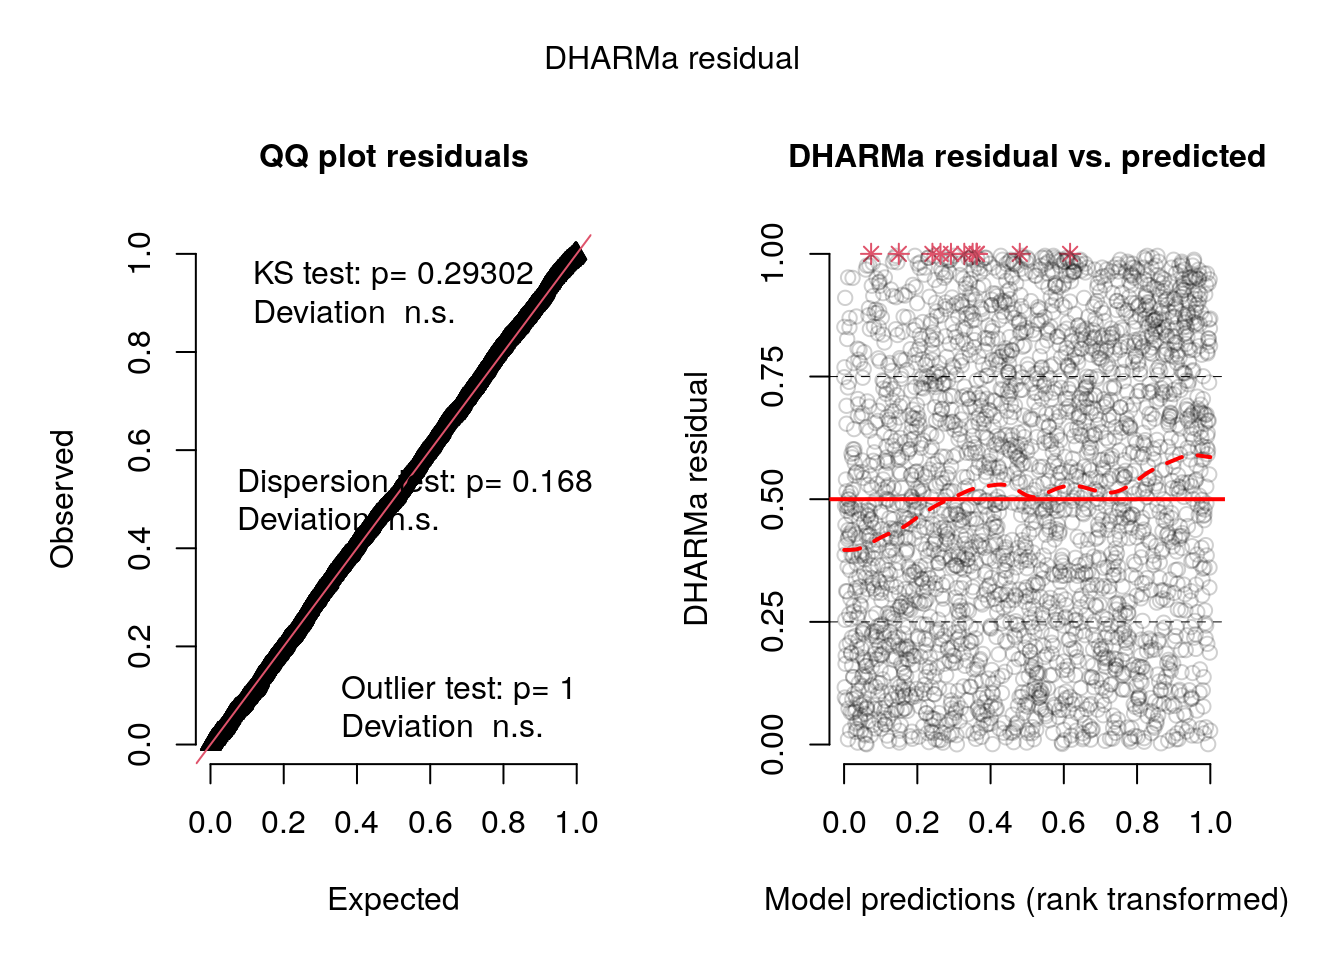
\includegraphics[keepaspectratio]{figure/unnamed-chunk-20-1.png}}

\subsubsection{Estimated marginal means}\label{estimated-marginal-means}

Lets consider marginal means between net types.

\begin{Shaded}
\begin{Highlighting}[]
\NormalTok{m.glmm.random2.hurdle.net }\OtherTok{\textless{}{-}} \FunctionTok{glmmTMB}\NormalTok{(}
\NormalTok{    nflounder }\SpecialCharTok{\textasciitilde{}}\NormalTok{ year }\SpecialCharTok{+}\NormalTok{ lat }\SpecialCharTok{+}\NormalTok{ long }\SpecialCharTok{+}\NormalTok{ distshore }\SpecialCharTok{+}\NormalTok{ area }\SpecialCharTok{+}\NormalTok{ chlorophyll }\SpecialCharTok{+}\NormalTok{ tempavg }\SpecialCharTok{+}\NormalTok{ tempstdev }\SpecialCharTok{+}\NormalTok{ sal }\SpecialCharTok{+}\NormalTok{ bod }\SpecialCharTok{+}\NormalTok{ nh3 }\SpecialCharTok{+}\NormalTok{ po4 }\SpecialCharTok{+}\NormalTok{ depth }\SpecialCharTok{+}\NormalTok{ net }\SpecialCharTok{+}\NormalTok{ (}\DecValTok{1} \SpecialCharTok{|}\NormalTok{ site}\SpecialCharTok{/}\NormalTok{net), }
    \AttributeTok{data =}\NormalTok{ df, }
    \AttributeTok{ziformula=}\SpecialCharTok{\textasciitilde{}}\NormalTok{.,}
    \AttributeTok{family=}\FunctionTok{truncated\_nbinom2}\NormalTok{()}
\NormalTok{)}
\FunctionTok{summary}\NormalTok{(m.glmm.random2.hurdle.net)}
\end{Highlighting}
\end{Shaded}

\begin{verbatim}
##  Family: truncated_nbinom2  ( log )
## Formula:          
## nflounder ~ year + lat + long + distshore + area + chlorophyll +  
##     tempavg + tempstdev + sal + bod + nh3 + po4 + depth + net +  
##     (1 | site/net)
## Zero inflation:             ~.
## Data: df
## 
##      AIC      BIC   logLik deviance df.resid 
##  12607.2  12825.8  -6266.6  12533.2     2687 
## 
## Random effects:
## 
## Conditional model:
##  Groups   Name        Variance Std.Dev.
##  net:site (Intercept) 0.07618  0.2760  
##  site     (Intercept) 0.70104  0.8373  
## Number of obs: 2724, groups:  net:site, 191; site, 74
## 
## Zero-inflation model:
##  Groups   Name        Variance Std.Dev.
##  net:site (Intercept) 0.09005  0.3001  
##  site     (Intercept) 0.47974  0.6926  
## Number of obs: 2724, groups:  net:site, 191; site, 74
## 
## Dispersion parameter for truncated_nbinom2 family (): 0.28 
## 
## Conditional model:
##               Estimate Std. Error z value Pr(>|z|)    
## (Intercept)  1.125e+02  2.674e+01   4.208 2.57e-05 ***
## year        -6.130e-02  1.253e-02  -4.893 9.95e-07 ***
## lat          2.436e-01  1.710e-01   1.424 0.154340    
## long         8.336e-02  1.250e-01   0.667 0.504755    
## distshore   -3.740e-01  7.193e-02  -5.200 2.00e-07 ***
## area        -1.803e-02  5.472e-02  -0.329 0.741826    
## chlorophyll -6.042e-02  6.015e-02  -1.005 0.315135    
## tempavg      6.471e-02  3.251e-02   1.991 0.046530 *  
## tempstdev    6.145e-05  4.511e-02   0.001 0.998913    
## sal         -8.518e-02  2.211e-02  -3.852 0.000117 ***
## bod          2.828e-01  2.217e-01   1.276 0.202061    
## nh3         -4.280e+00  4.288e+00  -0.998 0.318188    
## po4          1.242e-02  1.110e-02   1.119 0.263116    
## depth       -8.127e-02  8.344e-02  -0.974 0.330012    
## netBT       -2.305e-02  1.483e-01  -0.155 0.876487    
## netFyke      5.050e-02  1.322e-01   0.382 0.702464    
## ---
## Signif. codes:  0 '***' 0.001 '**' 0.01 '*' 0.05 '.' 0.1 ' ' 1
## 
## Zero-inflation model:
##               Estimate Std. Error z value Pr(>|z|)    
## (Intercept) -1.546e+02  2.624e+01  -5.891 3.84e-09 ***
## year         7.588e-02  1.247e-02   6.085 1.16e-09 ***
## lat         -4.906e-02  1.374e-01  -0.357  0.72097    
## long        -4.529e-01  1.058e-01  -4.280 1.87e-05 ***
## distshore    1.838e-01  5.686e-02   3.232  0.00123 ** 
## area        -2.822e-02  5.435e-02  -0.519  0.60356    
## chlorophyll  9.441e-02  5.436e-02   1.737  0.08240 .  
## tempavg     -2.844e-02  2.947e-02  -0.965  0.33439    
## tempstdev   -9.572e-02  4.217e-02  -2.270  0.02321 *  
## sal          7.959e-02  1.700e-02   4.683 2.83e-06 ***
## bod         -2.858e-01  1.928e-01  -1.482  0.13821    
## nh3          1.055e+00  3.363e+00   0.314  0.75369    
## po4          7.438e-04  9.325e-03   0.080  0.93642    
## depth        1.134e-01  6.514e-02   1.741  0.08175 .  
## netBT        2.647e-01  1.396e-01   1.895  0.05804 .  
## netFyke      1.037e-01  1.258e-01   0.824  0.40992    
## ---
## Signif. codes:  0 '***' 0.001 '**' 0.01 '*' 0.05 '.' 0.1 ' ' 1
\end{verbatim}

\begin{Shaded}
\begin{Highlighting}[]
\FunctionTok{emmeans}\NormalTok{(m.glmm.random2.hurdle.net,}\StringTok{"net"}\NormalTok{)}
\end{Highlighting}
\end{Shaded}

\begin{verbatim}
##  net  emmean    SE  df asymp.LCL asymp.UCL
##  BS     1.19 0.167 Inf     0.857      1.51
##  BT     1.16 0.188 Inf     0.793      1.53
##  Fyke   1.24 0.176 Inf     0.891      1.58
## 
## Results are given on the log (not the response) scale. 
## Confidence level used: 0.95
\end{verbatim}

\subsubsection{Variable selection with
drop1}\label{variable-selection-with-drop1}

Refit the model with various terms dropped.

\begin{Shaded}
\begin{Highlighting}[]
\FunctionTok{system.time}\NormalTok{(m.glmm.random2.hurdle.d1 }\OtherTok{\textless{}{-}} \FunctionTok{drop1}\NormalTok{(m.glmm.random2.hurdle,}\AttributeTok{test=}\StringTok{"Chisq"}\NormalTok{))}
\end{Highlighting}
\end{Shaded}

\begin{verbatim}
##    user  system elapsed 
## 250.071  12.708 248.697
\end{verbatim}

\begin{Shaded}
\begin{Highlighting}[]
\FunctionTok{print}\NormalTok{(m.glmm.random2.hurdle.d1)}
\end{Highlighting}
\end{Shaded}

\begin{verbatim}
## Single term deletions
## 
## Model:
## nflounder ~ year + lat + long + distshore + area + chlorophyll + 
##     tempavg + tempstdev + sal + bod + nh3 + po4 + depth + (1 | 
##     site/net)
##             Df   AIC    LRT  Pr(>Chi)    
## <none>         12603                     
## year         2 12666 67.016 2.803e-15 ***
## lat          2 12601  2.188 0.3349165    
## long         2 12616 16.602 0.0002483 ***
## distshore    2 12636 36.775 1.034e-08 ***
## area         2 12599  0.410 0.8147107    
## chlorophyll  2 12603  4.128 0.1269135    
## tempavg      2 12604  4.846 0.0886542 .  
## tempstdev    2 12604  4.661 0.0972639 .  
## sal          2 12632 32.729 7.816e-08 ***
## bod          2 12603  3.686 0.1583137    
## nh3          2 12600  1.087 0.5808045    
## po4          2 12600  1.307 0.5203431    
## depth        2 12603  4.024 0.1337202    
## ---
## Signif. codes:  0 '***' 0.001 '**' 0.01 '*' 0.05 '.' 0.1 ' ' 1
\end{verbatim}

Lets remove some of the variables (bod, nh3, po4).

\begin{Shaded}
\begin{Highlighting}[]
\NormalTok{final }\OtherTok{\textless{}{-}} \FunctionTok{glmmTMB}\NormalTok{(nflounder }\SpecialCharTok{\textasciitilde{}}\NormalTok{ year }\SpecialCharTok{+}\NormalTok{ lat }\SpecialCharTok{+}\NormalTok{ long }\SpecialCharTok{+}\NormalTok{ distshore }\SpecialCharTok{+}\NormalTok{ chlorophyll }\SpecialCharTok{+}\NormalTok{ tempavg }\SpecialCharTok{+}\NormalTok{ tempstdev }\SpecialCharTok{+}\NormalTok{ sal }\SpecialCharTok{+}\NormalTok{ depth }\SpecialCharTok{+}\NormalTok{ (}\DecValTok{1} \SpecialCharTok{|}\NormalTok{ site}\SpecialCharTok{/}\NormalTok{net), }
    \AttributeTok{data =}\NormalTok{ df, }
    \AttributeTok{ziformula=}\SpecialCharTok{\textasciitilde{}}\NormalTok{.,}
    \AttributeTok{family=}\FunctionTok{truncated\_nbinom2}\NormalTok{())}
\FunctionTok{summary}\NormalTok{(final)}
\end{Highlighting}
\end{Shaded}

\begin{verbatim}
##  Family: truncated_nbinom2  ( log )
## Formula:          
## nflounder ~ year + lat + long + distshore + chlorophyll + tempavg +  
##     tempstdev + sal + depth + (1 | site/net)
## Zero inflation:             ~.
## Data: df
## 
##      AIC      BIC   logLik deviance df.resid 
##  12593.0  12740.8  -6271.5  12543.0     2699 
## 
## Random effects:
## 
## Conditional model:
##  Groups   Name        Variance Std.Dev.
##  net:site (Intercept) 0.08427  0.2903  
##  site     (Intercept) 0.70174  0.8377  
## Number of obs: 2724, groups:  net:site, 191; site, 74
## 
## Zero-inflation model:
##  Groups   Name        Variance Std.Dev.
##  net:site (Intercept) 0.1120   0.3347  
##  site     (Intercept) 0.4647   0.6817  
## Number of obs: 2724, groups:  net:site, 191; site, 74
## 
## Dispersion parameter for truncated_nbinom2 family (): 0.278 
## 
## Conditional model:
##               Estimate Std. Error z value Pr(>|z|)    
## (Intercept) 119.527354  25.435578   4.699 2.61e-06 ***
## year         -0.062489   0.012236  -5.107 3.27e-07 ***
## lat           0.182753   0.148231   1.233    0.218    
## long          0.170123   0.100641   1.690    0.091 .  
## distshore    -0.371930   0.071585  -5.196 2.04e-07 ***
## chlorophyll  -0.063906   0.059707  -1.070    0.284    
## tempavg       0.062877   0.032362   1.943    0.052 .  
## tempstdev    -0.001606   0.043740  -0.037    0.971    
## sal          -0.092118   0.020512  -4.491 7.09e-06 ***
## depth        -0.090804   0.075929  -1.196    0.232    
## ---
## Signif. codes:  0 '***' 0.001 '**' 0.01 '*' 0.05 '.' 0.1 ' ' 1
## 
## Zero-inflation model:
##               Estimate Std. Error z value Pr(>|z|)    
## (Intercept) -164.69953   25.01589  -6.584 4.59e-11 ***
## year           0.07845    0.01216   6.449 1.12e-10 ***
## lat            0.03243    0.11729   0.276 0.782183    
## long          -0.48693    0.08346  -5.835 5.39e-09 ***
## distshore      0.19285    0.05665   3.404 0.000663 ***
## chlorophyll    0.08952    0.05390   1.661 0.096736 .  
## tempavg       -0.02442    0.02925  -0.835 0.403760    
## tempstdev     -0.10104    0.04091  -2.470 0.013511 *  
## sal            0.07914    0.01586   4.990 6.05e-07 ***
## depth          0.12938    0.05890   2.197 0.028055 *  
## ---
## Signif. codes:  0 '***' 0.001 '**' 0.01 '*' 0.05 '.' 0.1 ' ' 1
\end{verbatim}

\subsection{Conclusion}\label{conclusion}

The response variable nflounder is modeled using a truncated negative
binomial distribution with a log link function (Hurdle).

Truncated Negative Binomial model is a two part model, where the
zero-inflation model estimates the presence/absence; the conditional
model estimates the abundance.

The predictors in the both parts of the model include year, lat, long,
distshore, chlorophyll, tempavg, tempstdev, sal, and depth, along with a
random intercept for site/net.

\subsubsection{Random effect}\label{random-effect}

\paragraph{Conditional Model:}\label{conditional-model}

\begin{itemize}
\tightlist
\item
  net:site Group (Intercept): The variability in the response variable
  nflounder due to the grouping of nets within sites is relatively low,
  with a variance of 0.08427 and a standard deviation of 0.2903.
\item
  site Group (Intercept): The variability in nflounder due to different
  sites is higher compared to the net:site grouping, with a variance of
  0.70174 and a standard deviation of 0.8377.
\end{itemize}

\paragraph{Zero-Inflation Model:}\label{zero-inflation-model}

net:site Group (Intercept): The variability in the zero-inflation
component attributable to the grouping of nets within sites is moderate,
with a variance of 0.1120 and a standard deviation of 0.3347. site Group
(Intercept): The variability in zero-inflation due to different sites is
relatively higher, with a variance of 0.4647 and a standard deviation of
0.6817.

\subsubsection{Fixed Effects}\label{fixed-effects}

\paragraph{Conditional Model:}\label{conditional-model-1}

The predictor year is statistically significant (p \textless{} 0.001),
with a negative coefficient indicating a decrease in nflounder over
time. distshore and salinity also show significance (p \textless{} 0.001
and p \textless{} 0.05, respectively), with negative coefficients
implying a negative association with nflounder. Other predictors such as
latitude, longitude, chlorophyll, average temperature, temperature
standard deviation, and depth do not show statistically significant
associations with nflounder.

\paragraph{Zero-Inflation Model:}\label{zero-inflation-model-1}

Similar to the conditional model, year, latitude, longitude, distshore,
and salinity are statistically significant predictors (p \textless{}
0.001 or p \textless{} 0.05). temperature standard deviation also shows
significance (p \textless{} 0.05), but with a negative coefficient,
indicating a negative association with the zero-inflation component.

Overal, including random effects for site and net reduces AIC and
improves model fit, indicating that accounting for site-specific and
net-specific variability is important. Nested random effects (site/net)
further improve the model fit slightly compared to separate random
effects. The models indicate that both spatial (longitude, distance to
shore) and environmental (temperature, salinity, depth) variables
significantly influence flounder counts. Random effects for site and net
are crucial for capturing variability in the data, suggesting that there
are site-specific and gear-specific influences on flounder counts. The
year variable shows a strong temporal trend, which could indicate
changes in flounder population over time.

\subsection{References}\label{references}

Brooks ME, Kristensen K, van Benthem KJ, Magnusson A, Berg CW, Nielsen
A, Skaug HJ, Maechler M, Bolker BM (2017). ``glmmTMB Balances Speed and
Flexibility Among Packages for Zero-inflated Generalized Linear Mixed
Modeling.'' The R Journal, 9(2), 378--400.
\url{doi:10.32614/RJ-2017-066}.

\end{document}
